\renewcommand{\theequation}{\theenumi}
\begin{enumerate}[label=\thesection.\arabic*.,ref=\thesection.\theenumi]
\numberwithin{equation}{enumi}
\item The histogram for the above data is plotted in the fig. 
\begin{figure}[!ht]
\centering
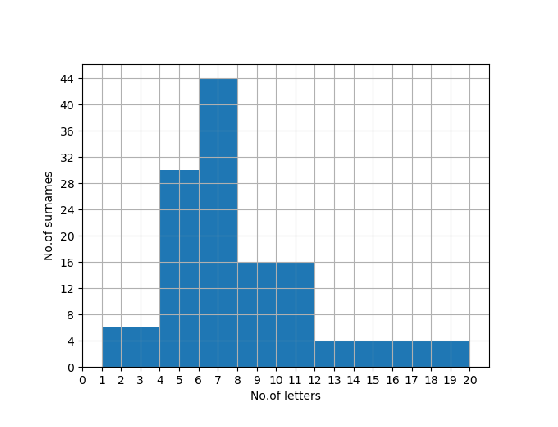
\includegraphics[width= \columnwidth]{./statistics/figs/Q45.eps}
\caption{Histogram of no.of surnames vs. no.of letters}
\end{figure}

\item From the graph, we can easily say that the maximum number of surnames is 44 which lies in the interval of 6 - 8.
\item Download the python code for the figure from 
\begin{lstlisting}
statistics/codes/Q45.py
\end{lstlisting}

\end{enumerate}